%! Author = Jean-Luc MUPASA KALUNGA
%
% Article (English, default version), translated from supply_chain_resilience_fr.tex, the working version.
% Same structure, labels, tables (tables_en/) and figures (*_en.pdf) as the French version.

\documentclass[11pt,a4paper]{article}

% Base packages
\usepackage[utf8]{inputenc}
\usepackage[T1]{fontenc}
\usepackage{lmodern}
\usepackage[english]{babel}
\usepackage{microtype}
\usepackage[a4paper,margin=2.2cm]{geometry}
\usepackage{amsmath,amssymb,mathtools,amsthm}
\usepackage{graphicx}
\usepackage{booktabs}
\usepackage{array}
\usepackage{tabularx}
\usepackage{multirow}
\usepackage{makecell}
\usepackage{enumitem}
\usepackage{xcolor}
\usepackage{float}
\usepackage{caption}
\usepackage{subcaption}

% Pseudocode
\usepackage{algorithm}
\usepackage{algpseudocode}

% References and links
\usepackage[hyphens]{url}
\usepackage{hyperref}
\usepackage[nameinlink,capitalise]{cleveref}

\hypersetup{
  colorlinks=true,
  linkcolor=blue!55!black,
  citecolor=blue!55!black,
  urlcolor=blue!65!black,
  pdftitle={Machine Learning-Based Delivery Delay Prediction for Supply Chain Resilience},
  pdfauthor={Jean-Luc MUPASA KALUNGA}
}

% Captions and tables
\captionsetup{font=small,labelfont=bf}
\setlist[itemize]{leftmargin=1.5em,itemsep=2pt,topsep=4pt}
\setlist[enumerate]{leftmargin=1.7em,itemsep=2pt,topsep=4pt}
\renewcommand{\arraystretch}{1.15}

\pagestyle{plain}

% Table rows generated by tables.py (\input cannot be used inside a tabular)
\makeatletter\newcommand{\tablerows}[1]{\@@input #1 }\makeatother
% Pipeline diagram (Figure 1)
\usepackage{tikz}
\usetikzlibrary{positioning,arrows.meta,fit,backgrounds,calc}

% Math macros
\newcommand{\E}{\mathbb{E}}
\newcommand{\Prob}{\mathbb{P}}
\newcommand{\ind}{\mathbf{1}}
\newcommand{\Preci}{\mathrm{Prec}}
\newcommand{\Rapp}{\mathrm{Rec}}

% Definition environments
\theoremstyle{definition}
\newtheorem{definition}{Definition}
\newtheorem{contrainte}{Constraint}

% Title and authors
\title{\textbf{Machine Learning-Based Delivery Delay Prediction for Supply Chain Resilience}}

\author{%
\begin{tabular}{c}
Mupasa Kalunga Jean-Luc$^{1}$ \qquad Mpyana Mwamba Merlec$^{2}$\\[0.5em]
{\small $^{1}$Faculty of Computer Science, Don Bosco University of Lubumbashi (UDBL), Lubumbashi, DRC}\\
{\small $^{2}$Department of Computer Science, Korea University, Seoul, South Korea}\\[0.3em]
{\small\texttt{16mk293@esisalama.org; mlecjm@korea.ac.kr}}
\end{tabular}%
}
\date{}


\begin{document}

\maketitle

\begin{abstract}
Machine learning models that predict delivery delays are usually evaluated by splitting the data at random between training and test sets, which assumes a distribution that is stable over time. On two public datasets, DataCo and Olist, we compare this random split with a chronological split that reproduces deployment conditions, for the classification and the regression of delays, using a linear baseline, a random forest and XGBoost tuned with an equal budget and without information leakage. On Olist, where the prevalence of delays drifts, random evaluation strongly overestimates performance: the area under the precision-recall curve of XGBoost rises from 0.067 under deployment conditions to 0.279, and the area under the ROC curve, which does not depend on prevalence, falls as well. When a missed delay costs five times as much as a false alarm, random evaluation promises a saving of 19.6\% over the best policy without a model, whereas the model actually costs 22.3\% more; on DataCo, where prevalence is stable, the two protocols agree. The optimism gap therefore depends on the stationarity of the data and can reverse the decision to deploy an alert system, which calls for evaluating these models in time order.
\end{abstract}

\noindent\textbf{Keywords:} supply chain resilience; delivery delay prediction; temporal validation; distribution shift; gradient boosting; hyperparameter optimization.

% ============================================================================
% Section 1: Introduction
% ============================================================================
\section{Introduction}
\label{sec:intro}

On-time delivery is one of the pillars of supply chain performance. It determines customer satisfaction, inventory availability and the planning of warehouse resources. A delay never stays local: it propagates downstream, ties up inventory, causes stockouts and can trigger contractual penalties. Its cost is measurable. For the firm, the public announcement of a production or shipping delay comes with an average abnormal drop of 10.28\% in the share price over the two days around the announcement, according to 519 announcements by US-listed firms between 1989 and 2000 \cite{hendricks2003effect}. For the customer relationship, at an online retailer, loyal customers whose orders arrive one to seven days late subsequently reduce the frequency and amount of their purchases more than a control group served on time \cite{rao2011failure}. The resilience of a supply chain is therefore not limited to its ability to absorb a disruption once it has occurred; it also requires anticipating the disruption, so as to give the manager time to act: choose another carrier, reallocate inventory or warn the customer.

Anticipating a delay is difficult, because its causes are many, interdependent and changing: weather, port congestion, customs formalities, uneven carrier reliability, the state of the infrastructure. Their effects do not simply add up, and their relative weight changes over time (seasonality, one-off disruptions, network or carrier changes). A linear model captures these interactions poorly, which motivates the use of machine learning, and in particular of ensembles of decision trees \cite{breiman2001random,friedman2001greedy,chen2016xgboost}, which we nonetheless compare with a linear baseline.

A recent literature applies supervised learning to the prediction of delays and logistics risks, with models ranging from classical regressions to deep networks \cite{rezki2024machine,douaioui2024deep,zogaan2025leveraging,widayanti2026predicting}. It shows that a model trained on the shipment history can produce actionable alerts. How these performances are \emph{estimated}, however, is seldom discussed. Splitting the observations at random into training and test sets assumes that the data are independent and identically distributed: the model is then evaluated on shipments whose close neighbours in time it has seen during training. Supply chains do not satisfy this assumption, because they undergo seasonal variations, regime changes and structural shifts. In other fields, studies show that this kind of split can lead to overly optimistic estimates: malware detection \cite{pendlebury2019tesseract}, chemical modelling \cite{sheridan2013time}, time series forecasting \cite{cerqueira2020evaluating,hewamalage2023forecast}. The size of the gap, however, depends on the stationarity of the data \cite{cerqueira2020evaluating}: it must therefore be measured, not assumed. More generally, information leakage, temporal leakage included, is among the causes of irreproducibility in applied machine learning \cite{kapoor2023leakage,kaufman2012leakage}. To our knowledge, the effect of the evaluation protocol has not been studied systematically for delivery delay prediction, on several public datasets.

The problem takes two complementary forms. \emph{Classification} indicates whether a delivery will be late and triggers the alert; \emph{regression} indicates by how many days, which allows the response to be sized (inventory to reallocate, replacement carrier, message to the customer). A manager who knew only whether a delay will occur could not tell whether to act for one day or for ten.

This article focuses on the following question: \emph{to what extent does the evaluation protocol affect the estimated reliability of machine learning models for delivery delay prediction, when they face a change over time in the data distribution?} It breaks down into two sub-questions:
\begin{description}[leftmargin=2.2em,style=nextline]
  \item[RQ1] Is the degradation observed under temporal evaluation found on real and independent datasets?
  \item[RQ2] What are the consequences of this degradation for operational decisions in response to delays?
\end{description}
Our working hypothesis is that evaluation by random split overestimates the performance actually obtained in deployment. This hypothesis is tested, not assumed, in what follows. We rely on two public datasets: DataCo Smart Supply Chain \cite{constante2019dataco}, the main dataset and a reference in the literature, and Olist Brazilian E-Commerce \cite{olist2018brazilian}, an independent dataset whose structure and prevalence of delays differ.

The contributions of this article are threefold:
\begin{enumerate}[label=(\roman*)]
  \item \textbf{A rigorous comparison of models.} We compare a regularized linear baseline, the random forest and XGBoost, whose hyperparameters are optimized with Optuna, on the dual task of classification and regression, under a protocol that rules out any information leakage. This comparison underpins the two other contributions.
  \item \textbf{A quantification of the effect of the evaluation protocol.} We compare the random split and the chronological split, measure the optimism gap between them and break it down by period. We translate its operational consequences through a cost-benefit analysis based on cost assumptions declared as illustrative.
  \item \textbf{A check of cross-dataset generalization.} We repeat the experiment on DataCo and then on Olist, two independent datasets, to establish whether the observed gap is a property of the problem or an artefact of a single file.
\end{enumerate}

The rest of the article is organized as follows. Section~\ref{sec:relwork} reviews related work and identifies the gap. Section~\ref{sec:formulation} formalizes the problem, the temporal causality constraint and the evaluation protocols. Section~\ref{sec:framework} describes the architecture and the methodology, Section~\ref{sec:design} the experimental setup, Section~\ref{sec:results} the results and their discussion, and Section~\ref{sec:conclusion} concludes.

% ============================================================================
% Section 2: Related work
% ============================================================================
\section{Related Work}
\label{sec:relwork}

We organize this review by theme rather than by paper: the prediction of delay risk by supervised learning (Section~\ref{sec:rw-supervise}), deep and temporal approaches (Section~\ref{sec:rw-profond}), model choice and hyperparameter optimization (Section~\ref{sec:rw-hpo}), evaluation protocols (Section~\ref{sec:rw-protocoles}) and datasets (Section~\ref{sec:rw-donnees}). Table~\ref{tab:litterature} summarizes them, and Section~\ref{sec:rw-lacune} derives the gap addressed by this article. For some works, only the abstract could be consulted \cite{rezki2024machine,widayanti2026predicting,bhuiyan2026deep,douaioui2024deep,sheridan2013time,pendlebury2019tesseract,hewamalage2023forecast}; we then use only what the abstract establishes.

\subsection{Supervised prediction of delay risk}
\label{sec:rw-supervise}

The works closest to our problem apply classical supervised models to the prediction of delays or logistics risk. Rezki and Mansouri \cite{rezki2024machine} compare seven algorithms (k-nearest neighbours, random forest, gradient boosting, linear regression, decision tree, logistic regression and support vector machine) on two tasks: the prediction of delivery delays and the classification of supplier performance. They conclude that ensemble methods give the best generalization error in regression, whereas logistic regression and gradient boosting stand out in classification. Widayanti et al. \cite{widayanti2026predicting} compare random forest, gradient boosting and support vector machine on more than 5{,}000 operational records covering 2018 to 2024; gradient boosting achieves the best accuracy. Sani et al. \cite{sani2023supply} predict backorder risk on 1.9 million weekly records covering eight weeks, with a LightGBM model whose hyperparameters are tuned by Bayesian optimization; they report an AUC of 0.957. Douaioui et al. address late delivery risk prediction with deep learning \cite{douaioui2024deep,douaioui2024enhancing}. In their journal article \cite{douaioui2024enhancing}, they use DataCo, cluster the order regions with the RIME metaheuristic and then predict one of four risk levels; the best model, a stack of networks, reaches an accuracy of 0.926. The dataset is thus shared with ours, but the target is not: our target is binary, which rules out a direct comparison of performance. Salari et al. \cite{salari2022realtime} predict the distribution of delivery time on 221{,}290 JD.com orders placed in March 2018, using quantile regression forests, including a cost-sensitive variant, and derive from it the date promised to the customer; their policy would increase sales volume by 3.7 to 6.1\% compared with JD.com's. To our knowledge, it is the work closest to ours through its regression task and its use of tree ensembles.

These works converge on one point: in the papers reviewed, tree ensembles frequently rank among the best models. They are not directly comparable with one another, however, because their data, targets and metrics differ: absolute and squared errors, precision, recall and F1 for Rezki and Mansouri, accuracy for Widayanti et al., AUC for Sani et al. Yet accuracy is not very informative when the positive class is a minority (Section~\ref{sec:metriques}).

\subsection{Deep and temporal approaches}
\label{sec:rw-profond}

A second family of works relies on deep architectures. Zogaan et al. \cite{zogaan2025leveraging} compare five networks (RNN, LSTM, GRU, CNN and multilayer perceptron) on four datasets published on Kaggle; to predict the on-time delivery of drugs (2{,}902 rows), the CNN reaches an accuracy of 99.3\%, against 95.18\% for Extra Trees and 93.12\% for the random forest. Jin \cite{jin2025attention} combines attention-based temporal convolutional networks with reinforcement learning to predict delays and optimize inventory; this preprint does not describe its data and compares its model only with an LSTM and ARIMA. Bhuiyan et al. \cite{bhuiyan2026deep} feed a deep model with macroeconomic indicators (GDP, inflation, trade, industrial output) and report an accuracy of 99.61\%; only their abstract is accessible. These approaches exploit the temporal dimension or exogenous signals, which is a potential advantage. But only Zogaan et al. compare themselves with tree ensembles, on a single dataset of a few thousand rows, and none of these three works states whether the training-test split is random or chronological. Their accuracies are therefore not comparable with one another, and how they were estimated remains unknown. Conversely, on 45 medium-sized tabular datasets, Grinsztajn et al. \cite{grinsztajn2022tree} show that tree ensembles remain superior to deep networks, even after an extensive hyperparameter search. Their benchmark, however, excludes time series and streaming data: this result supports the choice of trees on tabular data, but says nothing about the case where the distribution drifts. These two observations motivate our choice to study only tree ensembles and a linear baseline.

\subsection{Model choice and hyperparameter optimization}
\label{sec:rw-hpo}

Model choice and hyperparameter tuning belong to a separate methodological literature. Fazil et al. \cite{fazil2023comparative} find the random forest \cite{breiman2001random} superior to the support vector machine and to logistic regression for predicting rain from weather observations from 2008 to 2017; Latha et al. \cite{latha2024overview} review regression models and recommend $k$-fold cross-validation to select them. For tuning, random search is more efficient than grid search when few hyperparameters really matter \cite{bergstra2012random}, and Bayesian methods based on the tree-structured Parzen estimator \cite{bergstra2011algorithms}, implemented in Optuna \cite{akiba2019optuna}, steer the search using the trials already evaluated. Kee and Ho \cite{kee2025optimizing} compare grid search, random search and Optuna on 7{,}652 property transactions in Hong Kong (2010 to 2020), with gradient boosting and a random forest: Optuna is 6.77 to 108.92 times faster, for a virtually identical test $R^2$ (0.8549 against 0.8543 for gradient boosting). The number of trials given to each method is not reported and the experiment is not repeated, so the time difference is measured with an unknown budget; we therefore compare the three strategies with an equal number of trials and over several seeds (Sections~\ref{sec:hpo} and~\ref{sec:partitions}). The authors also recommend reporting metrics on the training set \emph{and} on the test set, to detect overfitting, which we adopt.

These papers justify our methodological choices, but they do not concern logistics, and none examines the effect of the split protocol on performance estimation. Yet the data of Fazil et al., like those of Kee and Ho, span about ten years, and Latha et al. recommend $k$-fold cross-validation without discussing time-ordered data.

\subsection{Evaluation protocols}
\label{sec:rw-protocoles}

\paragraph{In the delay literature.} The split protocol is rarely described explicitly. In the parts we consulted, the papers by Rezki and Mansouri and by Widayanti et al. do not state how the data are split between training and test. The full texts we read give at best proportions: 7:3 for Sani et al., 80/20 or 90/10 depending on the case for Zogaan et al., 70/30 for Kee and Ho, with five-fold cross-validation for tuning in Sani et al. and in Kee and Ho. None states whether the split is random or chronological, although the data of Sani et al. span eight weeks and those of Kee and Ho eleven years. Jin does not describe the split used, nor does the abstract of Bhuiyan et al. Douaioui et al. \cite{douaioui2024enhancing} mention training and test sets without describing how they were built. Salari et al. \cite{salari2022realtime} are the exception: they train their models on the orders of days 2 to 25 of the month and evaluate them on those of days 26 to 31, a chronological split, and set aside days 20 to 25 of the training period to validate their decision rule. They do not, however, compare this split with a random split: the effect of the protocol on estimated performance is not measured.

\paragraph{In other fields.} The question is better documented outside logistics. In chemistry, Sheridan \cite{sheridan2013time} shows that random splitting can inflate the estimated quality of a model, whereas chronological splitting gives a more realistic picture of its ability to predict new compounds. In malware detection, Pendlebury et al. \cite{pendlebury2019tesseract} attribute the inflated results reported in the literature to two biases, one spatial and one temporal; the latter comes from incorrect splits between training and test. They propose constraints on experimental design and a metric of performance over time. In time series forecasting, Cerqueira et al. \cite{cerqueira2020evaluating} compare variants of cross-validation, the holdout and prequential approaches on 174 real series and three synthetic ones: blocked cross-validation gives the best estimates on the 97 stationary series, whereas the holdout repeated over several periods wins on the 77 non-stationary series. Most methods overestimate the error there, but cross-validation without blocks tends to underestimate it, that is, to be optimistic. This caveat is essential, because it indicates that the optimism of random splitting depends on stationarity; we must therefore check it rather than assume it. Bergmeir and Benítez \cite{bergmeir2012use} find no practical effect of dependence on stationary series, to which their study is limited, and recommend blocked cross-validation together with a check of stationarity. Bergmeir et al. \cite{bergmeir2018note} show that standard cross-validation remains valid for autoregressive models whose lags are correctly specified, but that it underestimates the error when the model is badly misspecified. Neither condition holds by default for orders whose prevalence of delays varies over time. Hewamalage et al. \cite{hewamalage2023forecast} list the pitfalls of forecast evaluation, including random splitting, which does not preserve temporal order.

\paragraph{Information leakage and drift.} Information leakage is a broader problem. Kaufman et al. \cite{kaufman2012leakage} formalize it in data mining, and Kapoor and Narayanan \cite{kapoor2023leakage} propose a taxonomy for machine-learning-based science, which includes temporal leakage. Distribution shift has its own literature \cite{gama2014survey,morenotorres2012unifying}, on which we draw to formalize the problem (Section~\ref{sec:formulation}).

\begin{table}[!htbp]
\centering
\footnotesize
\caption{Summary of work on the prediction of delays and logistics risks. For papers whose abstract only was accessible or consulted, the mention ``in the abstract'' says so; the ``Protocol'' column is the one that reveals the gap addressed here. The last row, outside logistics, is included for its tuning methodology.}
\label{tab:litterature}
\newcolumntype{L}[1]{>{\raggedright\arraybackslash}p{#1}}
\begin{tabularx}{\textwidth}{@{}L{2.0cm}L{2.5cm}L{2.2cm}L{2.7cm}L{2.0cm}>{\raggedright\arraybackslash}X@{}}
\toprule
Reference & Data & Task & Models & Evaluation protocol & Reported metrics \\
\midrule
Rezki and Mansouri \cite{rezki2024machine} & Real data, origin and size not stated in the abstract & Delivery delay; supplier performance & KNN, RF, GB, linear regression, tree, logistic regression, SVM & Not described in the abstract & MAE, MSE, RMSE; precision, recall, F1 \\
Douaioui et al. \cite{douaioui2024enhancing} & DataCo & Delay risk level (four classes) & RIME clustering; GAN, CNN-LSTM, ensembles (bagging, boosting, stacking) & Not described & Accuracy, precision, F1, AUC, MSE, MAE, R\textsuperscript{2} \\
Salari et al. \cite{salari2022realtime} & JD.com, 221{,}290 orders (March 2018) & Delivery time distribution; promised date & Quantile regression forests, including a cost-sensitive variant & Chronological (days 2--25 / 26--31) & CRPS, pinball loss, log loss, Brier score; accuracy, F1, cost \\
Widayanti et al. \cite{widayanti2026predicting} & More than 5{,}000 records, 2018--2024 & Supply chain risk & RF, GB, SVM & Not described in the abstract & Accuracy \\
Zogaan et al. \cite{zogaan2025leveraging} & Four Kaggle datasets; delivery case: 2{,}902 rows & On-time delivery of drugs; three regression tasks & RNN, LSTM, GRU, CNN, perceptron; nine classical models, including RF & Proportions only (80/20, 90/10), order not stated & Accuracy, precision, recall; MAE, MSE, RMSE, MSLE \\
Sani et al. \cite{sani2023supply} & Backorders, 1.9 million records (8 weeks) & Backorder risk & LR, KNN, naive Bayes, tree, RF, XGBoost, LightGBM with Bayesian tuning & 7:3, order not stated; 5-fold cross-validation for tuning & Accuracy, precision, recall, AUC, computing time \\
Jin \cite{jin2025attention} & Not described (preprint) & Delay; inventory optimization & Attention TCN, reinforcement learning; LSTM, ARIMA & Not described & MAE, MSE, R\textsuperscript{2}, AUC \\
Bhuiyan et al. \cite{bhuiyan2026deep} & Not described in the abstract; macroeconomic indicators & Delivery delay risk & Deep learning & Not described in the abstract & Accuracy \\\midrule
Kee and Ho \cite{kee2025optimizing} & Property transactions, Hong Kong, 7{,}652 obs. (2010--2020) & Regression (price) & GBM, RF; grid, random, Optuna & 70\%/30\%, order not stated; 5-fold cross-validation for tuning & R\textsuperscript{2}, MAE, MedAE, MSE, MAPE, sMAPE, RMSE, RMSLE; training and test \\
\bottomrule
\end{tabularx}
\end{table}

\subsection{Datasets in the field}
\label{sec:rw-donnees}

The DataCo Smart Supply Chain dataset \cite{constante2019dataco} is public and citable; it is the one used by Douaioui et al. \cite{douaioui2024enhancing}. The Olist dataset \cite{olist2018brazilian}, also public, complements it with a different structure and prevalence of delays. Other works report relying on ``real data'' without describing them in their abstract \cite{rezki2024machine}, which limits the reproducibility and comparability of results. Using public, versioned and documented datasets is therefore a condition of our study.

\subsection{What is missing}
\label{sec:rw-lacune}

Three observations emerge from this review. First, tree ensembles are frequently the best performers in the works reviewed, but comparison across papers is limited by the diversity of data, targets and metrics. Second, the evaluation protocol is rarely described; when it is chronological, as in Salari et al. \cite{salari2022realtime}, it is not compared with a random split, although work in other fields shows that random splitting can overestimate performance under drift \cite{cerqueira2020evaluating}. Finally, no work known to us checks whether this gap recurs on several public and independent datasets. Our study addresses classification and regression together, compares the two protocols explicitly and repeats the analysis on DataCo and on Olist.

% ============================================================================
% Section 3: Mathematical framework
% ============================================================================
\section{Mathematical Framework}
\label{sec:formulation}

This section formalizes the problem to make it unambiguous and reproducible. It defines the two targets (Section~\ref{sec:notations}), the temporal causality constraint that separates admissible variables from leaking ones (Section~\ref{sec:causalite}), the evaluation protocols and drift (Section~\ref{sec:protocoles}), the loss functions (Section~\ref{sec:pertes}), the metrics (Section~\ref{sec:metriques}), the decision rule (Section~\ref{sec:decision}) and hyperparameter optimization (Section~\ref{sec:hpo}).

\subsection{Notation and targets}
\label{sec:notations}

Consider $n$ shipments indexed by $i \in \{1,\dots,n\}$. The unit of observation is the order or the order line, depending on the dataset (Section~\ref{sec:design}). Each shipment is associated with:
\begin{itemize}
  \item a prediction time $\tau_i$, at which the manager must have the alert;
  \item a promised delivery date $t_i^{p}$ (contractual or estimated date);
  \item an actual delivery date $t_i^{e}$, with $\tau_i < t_i^{e}$: prediction precedes delivery;
  \item a feature vector $\mathbf{x}_i \in \mathcal{X} \subseteq \mathbb{R}^{d}$, obtained after encoding the categorical variables.
\end{itemize}
The signed delay, in days, is
\begin{equation}
  \delta_i = t_i^{e} - t_i^{p}.
  \label{eq:delta}
\end{equation}
When only durations are available, as in DataCo, $\delta_i$ is the difference between the actual and the scheduled duration. A positive delay corresponds to a late delivery, a negative one to an early delivery. The two targets derive from $\delta_i$ defined by Equation~\eqref{eq:delta}:
\begin{align}
  y_i &= \ind\{\delta_i > 0\}, \label{eq:ycls}\\
  r_i &= \max(\delta_i, 0), \label{eq:yreg}
\end{align}
where $y_i \in \{0,1\}$ is the classification target (1 for a late delivery) and $r_i \ge 0$ the regression target, that is, the number of days of delay truncated at zero. Targets \eqref{eq:ycls} and \eqref{eq:yreg} are linked: $r_i > 0 \iff y_i = 1$, hence $r_i = y_i\,\delta_i$. We write $\pi = \Prob(y=1)$ for the prevalence of delays.

The target $r$ is not continuous on $\mathbb{R}_+$: it has a probability mass at zero (all on-time or early deliveries) and a continuous part for delays. Setting $p(\mathbf{x}) = \Prob(y=1 \mid \mathbf{x})$ and $m(\mathbf{x}) = \E[\delta \mid \mathbf{x},\, y=1]$, the conditional expectation of $r$ decomposes as
\begin{equation}
  \E[r \mid \mathbf{x}] = p(\mathbf{x})\, m(\mathbf{x}).
  \label{eq:decomp}
\end{equation}
Decomposition~\eqref{eq:decomp} motivates a two-model architecture: a classifier estimates $p$, and a regression model conditional on the delay estimates $m$, trained on the subset $\{i : y_i = 1\}$ where the target is strictly positive. We adopt this variant because it separates two problems of different nature, occurrence and magnitude, and because it avoids forcing a single regression model to fit a mass at zero. It also matches the decision: when an alert is issued, the date to announce depends on the magnitude of the delay given that it occurs, that is, on $m(\mathbf{x})$, and not on the expectation $\E[r \mid \mathbf{x}]$, which the mass at zero pulls downwards. A direct regression of $r$ on all observations would therefore not answer the question at hand; we do not retain it (Section~\ref{sec:articulation}).

\subsection{Temporal causality and information leakage}
\label{sec:causalite}

At time $\tau_i$, only part of the information about shipment $i$ is known. Let $a_{ij}$ be the time from which the $j$-th feature of shipment $i$ is known: the order date is known as soon as the order is placed, whereas the actual shipping duration is known only at delivery.

\begin{contrainte}[Availability]
\label{ctr:dispo}
A feature $j$ is admissible if it is known at prediction time for all shipments:
\begin{equation}
  \mathcal{J}_{\mathrm{adm}} = \bigl\{\, j \;:\; a_{ij} \le \tau_i \ \text{ for all } i \,\bigr\}.
  \label{eq:adm}
\end{equation}
Any feature outside $\mathcal{J}_{\mathrm{adm}}$ is a leaking variable and is excluded.
\end{contrainte}

Constraint~\ref{ctr:dispo}, which defines set~\eqref{eq:adm}, formally removes the variables posterior to $\tau_i$, such as the actual shipping duration or the final delivery status. It applies in the same way to both datasets. It transcribes the rule that Kaufman et al. call \emph{no-time-machine}: a variable is legitimate only if it is observable before the time at which the prediction of the target is requested \cite{kaufman2012leakage}. A variable that violates it falls into the category of illegitimate features in the taxonomy of Kapoor and Narayanan \cite{kapoor2023leakage}.

\paragraph{History features.} A feature computed from the past, such as the past delay rate of a seller or a shipping mode, requires particular care. For an entity $c_i$ (seller, region, shipping mode) and a window of width $w$, define the set of shipments \emph{already delivered} at time $\tau_i$:
\begin{equation}
  \mathcal{H}_i(w) = \bigl\{\, k \neq i \;:\; c_k = c_i,\ t_k^{e} \le \tau_i,\ \tau_i - t_k^{e} \le w \,\bigr\},
  \label{eq:hist}
\end{equation}
and the historical delay rate
\begin{equation}
  h_i =
  \begin{cases}
    \dfrac{1}{|\mathcal{H}_i(w)|} \displaystyle\sum_{k \in \mathcal{H}_i(w)} y_k & \text{if } |\mathcal{H}_i(w)| \ge n_{\min},\\[2ex]
    \text{missing value} & \text{otherwise.}
  \end{cases}
  \label{eq:taux}
\end{equation}
The condition in Equation~\eqref{eq:hist} bears on $t_k^{e} \le \tau_i$ (the delivery of $k$ is known before $\tau_i$) and not on $\tau_k < \tau_i$: a shipment placed earlier but still in transit has no known target, and including it would leak information. The threshold $n_{\min}$ in Equation~\eqref{eq:taux} avoids estimating a rate from too few observations; recent entities then receive a missing value, handled in the methodology (Section~\ref{sec:framework}).

\paragraph{Chronological split.} Fix a cut-off date $\tau^\star$.
\begin{contrainte}[Precedence between training and test]
\label{ctr:prec}
The training and test sets are
\begin{equation}
  \mathcal{D}_{\mathrm{ent}} = \{\, i : t_i^{e} \le \tau^\star \,\}, \qquad
  \mathcal{D}_{\mathrm{test}} = \{\, i : \tau_i \ge \tau^\star \,\}.
  \label{eq:split}
\end{equation}
\end{contrainte}
In \eqref{eq:split}, a shipment is thus used for training only if its target is known at $\tau^\star$, which reproduces real deployment conditions. The two sets are disjoint since $\tau_i < t_i^{e}$. Shipments such that $\tau_i < \tau^\star < t_i^{e}$, already predicted but not yet delivered at the cut-off date, belong to neither set; their number is reported in the experimental setup (Section~\ref{sec:design}).

Constraint~\ref{ctr:prec} bears on training examples, not on variables. Kaufman et al. show that Constraint~\ref{ctr:dispo} is not sufficient when the data are not stationary: training examples posterior to the evaluated targets create leakage, even if each of their variables is legitimate \cite{kaufman2012leakage}. The remedy they propose is precisely a separation by a cut-off in time. Kapoor and Narayanan classify as \emph{temporal leakage} any evaluation whose test set contains data earlier than the training set, when the model is used to predict a future event \cite{kapoor2023leakage}. A random split produces exactly this situation; this is what makes it the comparison protocol of this article.

\begin{contrainte}[Group integrity]
\label{ctr:groupes}
Let $g(i)$ be the group of observation $i$ (the order, when the unit is the order line). Two observations of the same group share the prediction time and are assigned to the same set.
\end{contrainte}
Without this constraint, a single order is scattered between training and test, which is direct leakage: Kapoor and Narayanan classify it among leakages due to non-independence between training and test, when the same units appear on both sides \cite{kapoor2023leakage}.

\subsection{Risk estimation, evaluation protocols and drift}
\label{sec:protocoles}

Let $\ell$ be a loss function. For a distribution $Q$ of $(\mathbf{X}, Y)$, the risk of a predictor $f$ is
\begin{equation}
  R_Q(f) = \E_{(\mathbf{X},Y)\sim Q}\bigl[\ell(f(\mathbf{X}), Y)\bigr].
  \label{eq:risque}
\end{equation}
Let $P_t$ be the joint distribution of $(\mathbf{X},Y)$ for the shipments whose prediction time is $t$, and $\mu$ the empirical distribution of prediction times over the study period. The implicit assumption of random splitting is \emph{stationarity}, $P_t = P$ for all $t$, with independent observations.

\paragraph{Two estimators.} In the random protocol, a test set $\mathcal{T}$ is drawn uniformly among the $n$ observations, and the model $f_{\mathcal{A}}$ is trained on the complement $\mathcal{A}$. In the chronological protocol, the model $f_{\mathrm{ent}}$ is trained on $\mathcal{D}_{\mathrm{ent}}$ and evaluated on $\mathcal{D}_{\mathrm{test}}$:
\begin{align}
  \widehat{R}_{\mathrm{rand}} &= \frac{1}{|\mathcal{T}|} \sum_{i\in\mathcal{T}} \ell\bigl(f_{\mathcal{A}}(\mathbf{x}_i), y_i\bigr), \label{eq:Ralea}\\
  \widehat{R}_{\mathrm{chr}} &= \frac{1}{|\mathcal{D}_{\mathrm{test}}|} \sum_{i\in\mathcal{D}_{\mathrm{test}}} \ell\bigl(f_{\mathrm{ent}}(\mathbf{x}_i), y_i\bigr). \label{eq:Rchr}
\end{align}
The test observations of the first protocol are spread over the whole period: they follow the mixture distribution $\bar{P} = \int P_t \,\mathrm{d}\mu(t)$. Those of the second follow the distribution of the period after the cut-off,
\begin{equation}
  P_{\mathrm{fut}} = \frac{1}{\mu\bigl((\tau^\star,\infty)\bigr)} \int_{(\tau^\star,\infty)} P_t \,\mathrm{d}\mu(t).
  \label{eq:Pfut}
\end{equation}
For a fixed predictor $f$ independent of the test sample, and for the risk defined by Equation~\eqref{eq:risque}, estimators \eqref{eq:Ralea} and \eqref{eq:Rchr} are unbiased for $R_{\bar{P}}(f)$ and $R_{P_{\mathrm{fut}}}(f)$ respectively. Under stationarity, $\bar{P} = P_{\mathrm{fut}} = P$ (distribution \eqref{eq:Pfut} coincides with the mixture) and both protocols target the same quantity. Under drift, they target two different quantities, and $R_{\bar{P}}(f) \neq R_{P_{\mathrm{fut}}}(f)$ in general.

The random protocol has a second source of optimism, independent of drift: the model $f_{\mathcal{A}}$ is trained on observations \emph{interleaved} with those of the test. When observations close in time are correlated (for instance during the same congestion episode), it interpolates instead of extrapolating.

\paragraph{Optimism gap.} For a score metric $M$ (higher is better), the optimism gap is
\begin{equation}
  \Delta_M = \widehat{M}_{\mathrm{rand}} - \widehat{M}_{\mathrm{chr}},
  \label{eq:delta-opt}
\end{equation}
and, for an error metric $E$ (lower is better), $\Delta_E = \widehat{E}_{\mathrm{chr}} - \widehat{E}_{\mathrm{rand}}$. Let $M_{\mathrm{dep}}(f)$ be the performance of $f$ trained on $\mathcal{D}_{\mathrm{ent}}$ and applied to shipments after $\tau^\star$: this is the performance under deployment conditions. The bias of a protocol $\pi$ is $B_\pi = \E[\widehat{M}_\pi] - M_{\mathrm{dep}}$. The chronological protocol reproduces these conditions, so $B_{\mathrm{chr}} \approx 0$ up to variance effects, and to a first approximation $\Delta_M \approx B_{\mathrm{rand}}$. Gap~\eqref{eq:delta-opt} thus measures the bias of random splitting; it is the quantity through which we operationalize the ``estimated reliability'' of the research question.

\paragraph{Drift profile.} To break the gap down by period, divide the test period into $Q$ consecutive periods of equal length (months in our experiments, Section~\ref{sec:partitions}) and let $\widehat{M}_q$ be the performance measured on the shipments of $\mathcal{D}_{\mathrm{test}}$ whose prediction time falls in period $q$. The sequence $q \mapsto \widehat{M}_q$ is the drift profile of the model; a breakdown corresponds to a drop of $\widehat{M}_q$ relative to validation performance.

\paragraph{Types of drift.} The joint distribution factorizes in two ways, as in Equation~\eqref{eq:facto}:
\begin{equation}
  P_t(\mathbf{x}, y) = P_t(y \mid \mathbf{x})\, P_t(\mathbf{x}) = P_t(\mathbf{x} \mid y)\, P_t(y).
  \label{eq:facto}
\end{equation}
Three forms of drift are then distinguished \cite{morenotorres2012unifying,gama2014survey}: covariate shift, when $P_t(\mathbf{x})$ varies and $P_t(y\mid\mathbf{x})$ stays fixed; prior probability shift, when $P_t(y)$ varies and $P_t(\mathbf{x}\mid y)$ stays fixed; concept shift, when $P_t(y\mid\mathbf{x})$ varies. We do not seek to identify the type of drift: we measure its consequences on performance estimation. Prior probability shift acts directly on some metrics (Section~\ref{sec:metriques}).

\subsection{Loss functions}
\label{sec:pertes}

\paragraph{Classification.} The model outputs a probability $\hat{p}(\mathbf{x}) \in (0,1)$. We minimize the weighted cross-entropy,
\begin{equation}
  \ell_w(y, \hat{p}) = -\bigl[\, w_1\, y \log \hat{p} + w_0\, (1-y) \log(1-\hat{p}) \,\bigr],
  \qquad w_1 = \frac{n}{2\,n_1}, \quad w_0 = \frac{n}{2\,n_0},
  \label{eq:logloss}
\end{equation}
where $n_c$ is the number of observations of class $c$. With the weights of Equation~\eqref{eq:logloss}, each class contributes the same total weight $n/2$, since $w_1 n_1 = w_0 n_0 = n/2$. Weighting has a marked effect only when the positive class is a minority; it is complemented by adjusting the decision threshold (Section~\ref{sec:imbalance}).

\paragraph{Regression.} Let $e_i = r_i - \hat{r}_i$ be the prediction error. The squared loss $e^2$ gives a quadratic weight to extreme delays. When delays have a heavy tail, which the exploratory analysis checks for each dataset (Section~\ref{sec:data-understanding}), we prefer the Huber loss \cite{huber1964robust}; this choice is made dataset by dataset in Section~\ref{sec:modeling},
\begin{equation}
  \ell_\kappa(e) =
  \begin{cases}
    \tfrac{1}{2}\, e^{2} & \text{if } |e| \le \kappa,\\[0.5ex]
    \kappa \bigl(|e| - \tfrac{1}{2}\kappa\bigr) & \text{otherwise.}
  \end{cases}
  \label{eq:huber}
\end{equation}
Loss~\eqref{eq:huber} is quadratic near zero and linear in the tails, hence less sensitive to extreme values. An alternative is to model $\tilde{r} = \log(1+r)$ and back-transform the prediction; this back-transformation, however, biases the conditional mean downwards (Jensen's inequality), which makes it less suitable for estimating the average magnitude of the delay.

\subsection{Evaluation metrics}
\label{sec:metriques}

\paragraph{Classification.} For a threshold $\theta$, the prediction is $\hat{y}_i(\theta) = \ind\{\hat{p}_i \ge \theta\}$. Let TP, FP, FN and TN denote the true positives, false positives, false negatives and true negatives. Then
\begin{align}
  \Preci &= \frac{\mathrm{TP}}{\mathrm{TP}+\mathrm{FP}}, &
  \Rapp &= \mathrm{TPR} = \frac{\mathrm{TP}}{\mathrm{TP}+\mathrm{FN}}, &
  \mathrm{FPR} &= \frac{\mathrm{FP}}{\mathrm{FP}+\mathrm{TN}}, \label{eq:prf}\\
  F_1 &= \frac{2\,\Preci\,\Rapp}{\Preci+\Rapp} = \frac{2\,\mathrm{TP}}{2\,\mathrm{TP}+\mathrm{FP}+\mathrm{FN}}. \label{eq:f1}
\end{align}

\emph{Why accuracy is set aside.} Accuracy $(\mathrm{TP}+\mathrm{TN})/n$ is dominated by the majority class: a classifier that always predicts ``on time'' reaches an accuracy of $1-\pi$ with zero recall. On a dataset where the prevalence of delays is low, this high score says nothing about the usefulness of the model.

\emph{ROC-AUC and PR-AUC.} The area under the ROC curve is the probability that a randomly drawn delay receives a higher score than a randomly drawn on-time delivery, ties counting for half; it does not depend on prevalence. Precision \eqref{eq:prf} does, as Bayes' formula shows:
\begin{equation}
  \Preci = \frac{\mathrm{TPR}\cdot\pi}{\mathrm{TPR}\cdot\pi + \mathrm{FPR}\cdot(1-\pi)}.
  \label{eq:prec-bayes}
\end{equation}
For the same point of the ROC curve, $\mathrm{TPR}=0.8$ and $\mathrm{FPR}=0.05$, precision is $0.8\cdot0.5/(0.8\cdot0.5+0.05\cdot0.5)\approx0.94$ if $\pi=0.5$, but only $0.8\cdot0.05/(0.8\cdot0.05+0.05\cdot0.95)\approx0.46$ if $\pi=0.05$. The ROC-AUC can thus look excellent while half the alerts are false alarms. The area under the precision-recall curve is approximated by the average precision,
\begin{equation}
  \mathrm{PR\text{-}AUC} \approx \sum_{k} \bigl(\Rapp_k - \Rapp_{k-1}\bigr)\,\Preci_k,
  \label{eq:ap}
\end{equation}
where the thresholds are the scores sorted in decreasing order; the value of a classifier without discriminating power is close to $\pi$. For these reasons, the PR-AUC \eqref{eq:ap} is more informative than the ROC-AUC when the positive class is a minority \cite{saito2015precision}; the $F_1$ score \eqref{eq:f1}, which combines the same precision and recall at a given threshold, complements the PR-AUC for the decision.

\emph{Link with drift.} If only the prevalence changes between two periods (the class-conditional distributions stay fixed), the point $(\mathrm{FPR},\mathrm{TPR})$ and the ROC-AUC are unchanged, whereas precision, PR-AUC and accuracy vary according to Equation~\eqref{eq:prec-bayes}. An optimism gap measured on these metrics can therefore come from a mere change in prevalence; we report the prevalence of each period to tell the cases apart.

\paragraph{Regression.} With $e_i = r_i - \hat{r}_i$ over a set of $N$ observations, we report the metrics of Equation~\eqref{eq:reg}:
\begin{equation}
  \mathrm{MAE} = \frac{1}{N}\sum_i |e_i|, \qquad
  \mathrm{RMSE} = \sqrt{\frac{1}{N}\sum_i e_i^{2}}, \qquad
  R^{2} = 1 - \frac{\sum_i e_i^{2}}{\sum_i (r_i-\bar{r})^{2}}.
  \label{eq:reg}
\end{equation}
The MAPE is undefined when $r_i = 0$, which is the case for all on-time deliveries; it can only be computed on the subset of delays $\{i : y_i = 1\}$, where $r_i > 0$. On this subset we prefer the sMAPE, whose denominator remains strictly positive:
\begin{equation*}
  \mathrm{sMAPE} = \frac{100}{n_1} \sum_{i:\,y_i=1} \frac{|e_i|}{\bigl(|r_i|+|\hat{r}_i|\bigr)/2}.
\end{equation*}

\paragraph{Variability.} For a metric $M$ computed over $S$ repetitions of the experiment, which differ by their random seed (Section~\ref{sec:partitions}), we report the mean and the standard deviation
\begin{equation*}
  \bar{M} = \frac{1}{S}\sum_{s=1}^{S} M_s, \qquad
  \mathrm{sd}(M) = \sqrt{\frac{1}{S-1}\sum_{s=1}^{S} \bigl(M_s-\bar{M}\bigr)^{2}},
\end{equation*}
never a single value.

\subsection{Decision rule and cost}
\label{sec:decision}

Let $c_{\mathrm{FN}}$ be the cost of an unreported delay and $c_{\mathrm{FP}}$ that of a false alarm. The cost of a threshold $\theta$ is
\begin{equation}
  C(\theta) = c_{\mathrm{FN}}\,\mathrm{FN}(\theta) + c_{\mathrm{FP}}\,\mathrm{FP}(\theta).
  \label{eq:cout}
\end{equation}
If the probabilities are well calibrated, predicting a delay costs $(1-p)\,c_{\mathrm{FP}}$ in expectation and predicting nothing costs $p\,c_{\mathrm{FN}}$; one therefore alerts as soon as $p \ge \theta^\star$, with
\begin{equation}
  \theta^\star = \frac{c_{\mathrm{FP}}}{c_{\mathrm{FP}} + c_{\mathrm{FN}}}.
  \label{eq:seuil}
\end{equation}
In practice, probabilities are rarely calibrated, so \eqref{eq:seuil} is not applied directly: the threshold is chosen by minimizing Equation~\eqref{eq:cout} on a validation set, never on the test set. As actual costs are not observed in our datasets, we treat them as illustrative assumptions. Comparing the cost obtained under the two protocols translates the optimism gap into a decision consequence and answers RQ2; as the two test sets do not have the same prevalence, this cost is expressed relative to that of a policy without a model (Section~\ref{sec:imbalance}).

\subsection{Hyperparameter optimization}
\label{sec:hpo}

Let $f_{\boldsymbol\lambda}$ be a model with hyperparameters $\boldsymbol\lambda \in \Lambda$. Tuning minimizes the validation risk, averaged over $K$ folds:
\begin{equation}
  \boldsymbol\lambda^\star = \arg\min_{\boldsymbol\lambda \in \Lambda} \; \frac{1}{K} \sum_{k=1}^{K} \mathcal{L}\bigl(f^{(k)}_{\boldsymbol\lambda};\, \mathcal{V}_k\bigr),
  \label{eq:hpo}
\end{equation}
where $f^{(k)}_{\boldsymbol\lambda}$ is trained on $\mathcal{T}_k$ and $\mathcal{L}$ denotes the optimized criterion. To respect Constraint~\ref{ctr:prec}, the folds are chronological, with an expanding window: for dates $s_1 < \dots < s_K$ taken within the training period,
\begin{equation}
  \mathcal{T}_k = \{\, i \in \mathcal{D}_{\mathrm{ent}} : t_i^{e} \le s_k \,\}, \qquad
  \mathcal{V}_k = \{\, i \in \mathcal{D}_{\mathrm{ent}} : s_k < \tau_i \le s_{k+1} \,\},
  \label{eq:plis}
\end{equation}
with $s_{K+1} = \tau^\star$. Tuning~\eqref{eq:hpo} thus relies on the chronological folds~\eqref{eq:plis}, so that internal validation follows the same principle as external evaluation. With random folds, hyperparameter selection would itself introduce an optimism bias. The random protocol serves as the comparator, with folds drawn at random and grouped (Constraint~\ref{ctr:groupes}).

Three search strategies are compared. Grid search evaluates the Cartesian product of predefined values. Random search draws $\boldsymbol\lambda$ from given distributions \cite{bergstra2012random}. The tree-structured Parzen estimator (TPE) \cite{bergstra2011algorithms}, used by Optuna \cite{akiba2019optuna}, proceeds sequentially: after $m$ trials $(\boldsymbol\lambda_j, v_j)$, where $v_j$ is the value of the criterion, one sets $v^\star$ as a quantile $\gamma$ of the observed values and models two densities,
\begin{equation}
  \ell(\boldsymbol\lambda) = p(\boldsymbol\lambda \mid v < v^\star), \qquad g(\boldsymbol\lambda) = p(\boldsymbol\lambda \mid v \ge v^\star).
  \label{eq:tpe}
\end{equation}
The next trial maximizes the ratio $\ell(\boldsymbol\lambda)/g(\boldsymbol\lambda)$ of densities \eqref{eq:tpe}, which amounts to maximizing the expected improvement \cite{bergstra2011algorithms}.

The three strategies receive the same budget of $B = 30$ trials per study, a study being a combination of dataset, task, model, protocol and seed. The grid is built to have exactly $B$ points; random search and TPE each evaluate $B$ configurations, the first ten being drawn at random for TPE, as Optuna does by default. With an equal budget, the comparison bears on the quality of the selected hyperparameters and not on the number of evaluations given to each method, which removes the limitation noted in Kee and Ho (Section~\ref{sec:rw-hpo}).

% ============================================================================
% Section 4: Proposed architecture and methodology
% ============================================================================
\section{Proposed Architecture and Methodology}
\label{sec:framework}

Our approach follows the six phases of the CRISP-DM process \cite{wirth2000crisp}: business understanding, data understanding, data preparation, modelling, evaluation and deployment. This section describes the first four; evaluation and deployment are covered in Sections~\ref{sec:design} and~\ref{sec:results}.

\subsection{Overview}
\label{sec:pipeline}

Figure~\ref{fig:pipeline} summarizes the approach. The first two phases set the objective, the costs and the targets; preparation produces, once and without leakage, the features shared by both protocols. The pipeline then splits in two: each protocol partitions the same orders, tunes the models on its own folds and evaluates them on its own test set. Evaluation confronts the two estimates, and the decision rule translates their gap into cost.

\begin{figure}[!htbp]
\centering
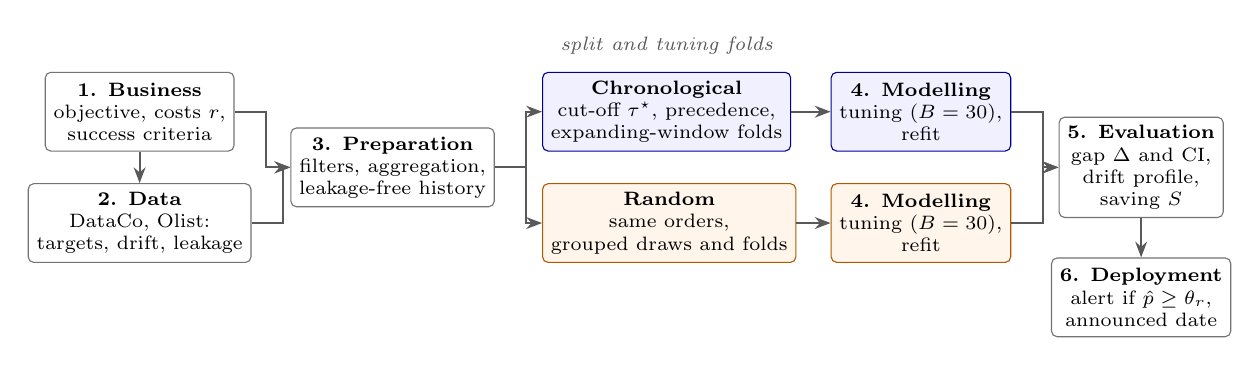
\begin{tikzpicture}[
  font=\scriptsize,
  box/.style={draw=black!55, rounded corners=2pt, align=center, inner sep=3pt, minimum height=10mm, fill=white},
  chrono/.style={box, draw=blue!60!black, fill=blue!6},
  alea/.style={box, draw=orange!70!black, fill=orange!8},
  note/.style={font=\scriptsize\itshape, text=black!65, align=center},
  arr/.style={-{Stealth[length=2mm]}, thick, black!65},
]
\node[box] (metier) {\textbf{1. Business}\\objective, costs $r$,\\success criteria};
\node[box, below=4mm of metier] (donnees) {\textbf{2. Data}\\DataCo, Olist:\\targets, drift, leakage};
\node[box, anchor=west] (prep) at ($(metier.east)!0.5!(donnees.east) + (6mm,0)$) {\textbf{3. Preparation}\\filters, aggregation,\\leakage-free history};
\node[chrono, anchor=south west] (pchr) at ($(prep.east) + (6mm,2mm)$) {\textbf{Chronological}\\cut-off $\tau^\star$, precedence,\\expanding-window folds};
\node[alea, anchor=north west] (pale) at ($(prep.east) + (6mm,-2mm)$) {\textbf{Random}\\same orders,\\grouped draws and folds};
\coordinate (col) at ($(pchr.east) + (5mm,0)$);
\node[chrono, anchor=west] (mchr) at (col |- pchr) {\textbf{4. Modelling}\\tuning ($B = 30$),\\refit};
\node[alea, anchor=west] (male) at (col |- pale) {\textbf{4. Modelling}\\tuning ($B = 30$),\\refit};
\node[box, anchor=west] (eval) at ($(mchr.east)!0.5!(male.east) + (6mm,0)$) {\textbf{5. Evaluation}\\gap $\Delta$ and CI,\\drift profile,\\saving $S$};
\node[box, below=5mm of eval] (decision) {\textbf{6. Deployment}\\alert if $\hat p \ge \theta_r$,\\announced date};
\draw[arr] (metier) -- (donnees);
\draw[arr] (metier.east) -- ++(4mm,0) |- (prep.west);
\draw[arr] (donnees.east) -- ++(4mm,0) |- (prep.west);
\draw[arr] (prep.east) -- ++(4mm,0) |- (pchr.west);
\draw[arr] (prep.east) -- ++(4mm,0) |- (pale.west);
\draw[arr] (pchr.east) -- (pchr.east -| mchr.west);
\draw[arr] (pale.east) -- (pale.east -| male.west);
\draw[arr] (mchr.east) -- ++(4mm,0) |- (eval.west);
\draw[arr] (male.east) -- ++(4mm,0) |- (eval.west);
\draw[arr] (eval) -- (decision);
\node[note, above=1mm of pchr] {split and tuning folds};
\end{tikzpicture}
\caption{The approach along the six phases of CRISP-DM. After preparation, the pipeline splits in two: both protocols bear on the same orders and differ only in how they are divided; evaluation measures the gap between their estimates and the decision rule translates it into cost.}
\label{fig:pipeline}
\end{figure}

\subsection{Business understanding}
\label{sec:business}

\paragraph{Decision objective.} We take the viewpoint of a retailer's customer service. The prediction time $\tau_i$ of Section~\ref{sec:notations} is set at the time of the order: it is the first moment at which the shipment exists in the information system, and the one that leaves the most time to act. When a delay is predicted, the chosen action is to warn the customer and announce a new delivery date. We prefer this action to a logistics action, such as changing the shipping mode or reminding the seller, for two reasons. First, it is available in both datasets, whereas the logistics levers differ: DataCo describes a shipping mode, Olist a seller. The same decision problem thus applies to both datasets, which conditions the comparison made in Section~\ref{sec:results}. Second, warning the customer does not change the actual delivery date: the target remains observed without any effect of the intervention, which would not be the case if the alert triggered a change of carrier.

\paragraph{Role of the two tasks.} The decision has two parts, which correspond to the two targets defined in Section~\ref{sec:notations}. The classifier estimates the probability of delay $p(\mathbf{x})$ and triggers the alert when $\hat{p}(\mathbf{x}_i) \ge \theta$. The conditional regression model estimates $m(\mathbf{x})$, the expected magnitude of the delay when it occurs (Equation~\eqref{eq:decomp}); in case of an alert, the date announced to the customer is
\begin{equation}
  \hat{t}_i = t_i^{p} + \hat{m}(\mathbf{x}_i).
  \label{eq:date-annoncee}
\end{equation}
Classification decides whether to act; regression determines what to announce. The magnitude itself has a cost: the longer the delay, the larger the drop in subsequent purchases \cite{rao2011failure}. It is this second piece of information that distinguishes a useful message, which lets the customer reorganize the reception, from an empty warning. The contribution of regression nevertheless depends on the dispersion of delays: on DataCo, where they range from one to four days (Section~\ref{sec:design}), it is necessarily limited. How the two models fit together is detailed in Section~\ref{sec:articulation}.

\paragraph{Cost of errors.} A false negative, that is, an unannounced delay, exposes the retailer to a complaint, to handling by customer service and to a loss of trust. A false positive, that is, a delay announced wrongly, costs a useless message and can also erode the customer's trust. The literature confirms these two costs and their asymmetry. Across more than 11 million purchases on a large e-commerce platform, a deviation from the promised date lowers the product rating by 0.4 points on average for a delay, and by 0.2 points for an early delivery \cite{nozari2026please}. A wrongly issued alert postpones the announced date: if the parcel arrives on the original date, it arrives early with respect to the new one. In fast delivery, a delay lengthens the time before repurchase more than an early delivery of the same size shortens it \cite{harter2025effect}. The stakes go beyond the rating: across more than 15 million orders on the Tmall platform, bringing three-day deliveries down to two days would increase the daily sales of third-party sellers by 13.3\% \cite{deshpande2023logistics}. We therefore assume $c_{\mathrm{FN}} > c_{\mathrm{FP}}$. Neither dataset records these costs: we treat them as illustrative assumptions, through the ratio $r = c_{\mathrm{FN}}/c_{\mathrm{FP}}$. Rather than fixing a single value, we study $r \in \{1, 2, 5, 10\}$, which correspond, for calibrated probabilities, to the thresholds $\theta^\star = 1/(1+r)$ of Equation~\eqref{eq:seuil}, namely 0.50, 0.33, 0.17 and 0.09; the value $r = 5$ is the main scenario. In line with Section~\ref{sec:decision}, the threshold is chosen for each value of $r$ by minimizing the cost $C(\theta)$ on the validation set, never on the test set. A conclusion that holds over this whole range does not depend on a particular cost assumption.

\paragraph{Success criteria.} They are set before any experiment. The main metric is the PR-AUC in classification and the MAE in regression, for the reasons given in Section~\ref{sec:metriques}. A model is deemed useful if its PR-AUC exceeds both the prevalence of the dataset, which is the value of a classifier without discriminating power, and that of the linear baseline. The optimism gap $\Delta_M$ of Equation~\eqref{eq:delta-opt} is considered a finding if its interval computed over five random seeds excludes zero (Equation~\eqref{eq:ic-delta}, Section~\ref{sec:partitions}). The chronological split rule is given in Section~\ref{sec:design}.

\subsection{Data understanding}
\label{sec:data-understanding}

The exploration of the two datasets has three goals: rebuild the targets of Section~\ref{sec:notations} and check their consistency, identify the variables that are not known at prediction time, and describe how the data change over time. The volumes and prevalences retained appear in Table~\ref{tab:donnees} (Section~\ref{sec:design}). These figures are produced by the data preparation script, which writes them to a summary file for each dataset, together with the diagnostics of this section, recomputed from the raw data.

\paragraph{Granularity and targets.} In DataCo, a row corresponds to an ordered item; an order has 2.75 rows on average, and the delay, the shipping mode and the order date are constant within an order. The delay $\delta_i$ is the difference between the actual and the scheduled shipping durations. The target thus rebuilt matches the dataset's \texttt{Late\_delivery\_risk} indicator on all non-cancelled rows. The 7{,}754 cancelled rows (statuses \texttt{CANCELED} and \texttt{SUSPECTED\_FRAUD}) are the exception: the indicator is always zero there, although no delivery took place, and contradicts the rebuilt target on 4{,}423 of them. These rows are excluded, the target being undefined. In Olist, a row corresponds to an order; we keep only delivered orders whose delivery date is recorded, and measure $\delta_i$ in calendar days between the delivery date and the estimated date communicated to the customer.

\paragraph{Variables posterior to prediction.} Several DataCo variables are known only after delivery and reveal the target: the actual shipping duration, the delivery status, the risk indicator and the order status. The shipping date is one of them: its gap in calendar days from the order date gives back the actual duration on every row. In Olist, the dates of payment approval, handover to the carrier and delivery are posterior to the purchase. So is the deadline for handover to the carrier, although it is set by the platform: for 78\% of items, it falls at the same time of day as the payment approval, a whole number of days later. All these variables are excluded (Section~\ref{sec:preparation}).

\paragraph{Structure of the scheduled lead time.} In DataCo, the scheduled lead time is entirely determined by the shipping mode (0, 1, 2 or 4 days), and first-class shipments are always late. Orders are spread almost uniformly over the twenty-four hours of the day, night included. Delays are short, from one to four days. These regularities suggest an at least partly synthetic dataset; we take this into account when discussing the validity of our results. In Olist, the estimated date is specific to each order, and delays have a long tail: the median is 7 days, the maximum 188.

\paragraph{Change over time.} The two datasets change in different ways. In DataCo, the prevalence of delays stays between 56.5 and 58.7\% from one quarter to the next, but the structure of orders changes from October 2017: an order has a single row instead of three, and the number of distinct products sold each month, between 42 and 87 before, falls to between 8 and 20. The distribution of the variables thus changes while the prevalence stays stable. In Olist, conversely, the prevalence varies from 3.4 to 12.9\% depending on the quarter, with a peak between October 2017 and March 2018. These two situations are reminiscent of covariate shift and prior probability shift, respectively (Section~\ref{sec:protocoles}); in line with that section, we do not derive a formal identification of the type of drift from them, but they suggest a larger gap between protocols on Olist.

\paragraph{End-of-period censoring.} The Olist extract contains only the orders already delivered at the time it was built. Orders placed shortly before that date therefore appear only if they were delivered quickly: the mean delivery time, still 8.0 days for purchases in the week of 6 August 2018, falls to 5.0 and then 1.8 days over the last two weeks of purchases. Keeping these orders would bias the prevalence downwards at the end of the period, that is, in the chronological test set. We therefore set the end of observation at the last order approval present in the data, 3 September 2018, and exclude purchases made in the 29 days before it, 29 days being the 95th percentile of delivery time. We also exclude the 267 orders from 2016, too few to represent that year.

\subsection{Data preparation}
\label{sec:preparation}

Preparation distinguishes two kinds of operations. Deterministic operations, which rely on no statistic of the data (filters, target construction, column removal, aggregation, date features, split), are applied once and for all by the preparation script. Learned operations, such as the imputation of missing values or the encoding of categorical variables, are instead embedded in the model and fitted on the training set of each split only (Section~\ref{sec:modeling}): applying them to the whole dataset would leak information from the test set into training \cite{kapoor2023leakage}. Table~\ref{tab:preparation} summarizes the data issues handled, linking them where relevant to the leakage taxonomy of Kapoor and Narayanan \cite{kapoor2023leakage}.

\begin{table}[!htbp]
\centering
\footnotesize
\caption{Data issues and treatments applied. The codes in brackets refer to the leakage taxonomy of Kapoor and Narayanan \cite{kapoor2023leakage}.}
\label{tab:preparation}
\newcolumntype{L}[1]{>{\raggedright\arraybackslash}p{#1}}
\begin{tabularx}{\textwidth}{@{}L{2.9cm}L{3.6cm}L{4.0cm}>{\raggedright\arraybackslash}X@{}}
\toprule
Issue & Diagnosis & Treatment & Impact \\
\midrule
Cancelled orders (DataCo) & 7{,}754 rows without delivery; the delay indicator is zero there & Rows excluded & 172{,}765 rows, 62{,}897 orders \\
Undelivered orders (Olist) & Status other than delivered, or missing delivery date & Orders excluded & 2{,}971 orders removed \\
Year 2016 (Olist) & 267 orders, too few to represent the year & Orders excluded & Period from January 2017 \\
End-of-period censoring (Olist) & Only orders already delivered appear in the extract & Purchases in the 29 days before the last approval excluded & 5{,}209 orders removed; 90{,}994 remain \\
Variables posterior to prediction [L2] & Actual duration, statuses, dates of shipping, approval, handover to the carrier and delivery & Variables excluded (Constraint~\ref{ctr:dispo}) & No variable known after prediction time \\
Uninformative columns (DataCo) & Empty, constant or very incomplete columns, exact copies of other columns, personal data & Columns excluded & 15 columns removed, in addition to the 5 posterior variables \\
Duplicates [L1.4] & No duplicate row & None & -- \\
Several items per order (Olist) & 10\% of orders have several items, 1.3\% several sellers & Aggregation by order; main item = most expensive; distance = maximum over items & One row per order \\
Impossible values (Olist) & Weight of 0\,g, zero instalments & Replaced by missing values & Handled like other missing values \\
Missing values [L1.2] & Olist: category (1{,}332 orders), distance (453), weight (19), instalments (2); DataCo: postcode (3) & Imputation learned on training, within the model & No test information in the imputation \\
Rows of the same order (DataCo) [L3.2] & 2.75 rows per order, shared target & Split grouped by order (Constraint~\ref{ctr:groupes}) & No order shared between training and test \\
Orders in transit at the cut-off [L3.1] & Placed before the cut-off, delivered after: target unknown at the cut-off & Excluded from both sets (Constraint~\ref{ctr:prec}) & DataCo: 188 orders; Olist: 3{,}032, of which 24.9\% late \\
\bottomrule
\end{tabularx}
\end{table}

The last treatment in the table deserves a comment. A late order, by definition, takes longer to be delivered; it is therefore more likely to be still in transit at the cut-off date. On Olist, the orders thus set aside are late in 24.9\% of cases, against 6.9\% over the whole dataset. Keeping them in training would have raised its prevalence from 7.0 to 7.8\%, with targets that no deployed model could yet have observed. This is leakage through training examples in the sense of Kaufman et al. \cite{kaufman2012leakage}, which goes through no variable.

\paragraph{History features.} We complement the features of each order with the past delay rate of several entities, computed according to Equations~\eqref{eq:hist} and~\eqref{eq:taux} with a window $w = 90$ days and a threshold $n_{\min} = 10$. For Olist, the entities are the main seller, the customer's state and the link between the seller's state and the customer's state; for DataCo, which records neither seller nor carrier, they are the order region, the shipping mode and their combination. Each entity yields two features: the historical rate and the number of orders it is based on, which informs the model about its reliability. Algorithm~\ref{alg:historique} gives the computation. It involves only orders already delivered at prediction time: the value obtained is the one a manager could have computed at that moment, whatever the evaluation protocol. It is therefore run only once, before any split. On DataCo, the computation is done at the order level, so that an order with several rows counts only once.

\begin{algorithm}[!htbp]
\caption{Leakage-free historical delay rate of an entity}
\label{alg:historique}
\begin{algorithmic}[1]
\Require orders $i$ with prediction time $\tau_i$, delivery time $t_i^{e}$, delay $y_i$ and entity $c_i$; window $w$; threshold $n_{\min}$
\Ensure for each order, count $n_i = |\mathcal{H}_i(w)|$ and rate $h_i$
\For{each entity $c$}
  \State $L \gets$ the orders of $c$, sorted by increasing $t^{e}$; $S \gets$ the cumulative sums of their $y$
  \For{each order $i$ of $c$}
    \State $b \gets \#\{k \in L : t_k^{e} \le \tau_i\}$; $a \gets \#\{k \in L : t_k^{e} < \tau_i - w\}$ \Comment{binary search}
    \State $n_i \gets b - a$; $r_i \gets S_b - S_a$
    \If{$\tau_i - w \le t_i^{e} \le \tau_i$} \Comment{$k \neq i$: same-day delivery}
      \State $n_i \gets n_i - 1$; $r_i \gets r_i - y_i$
    \EndIf
    \State $h_i \gets r_i / n_i$ if $n_i \ge n_{\min}$, missing value otherwise
  \EndFor
\EndFor
\end{algorithmic}
\end{algorithm}

The computation is checked in two ways: on randomly drawn orders, by comparing the result with the direct computation of definition~\eqref{eq:hist}, and on hand-built cases (order still in transit, same-day delivery, window, threshold). The resulting features are informative on Olist: the prevalence of delays is 2.5 times higher in the top quartile of the customer state's historical rate than in the bottom quartile (11.4 against 4.5\%), and 2.8 times for the link between states (12.0 against 4.3\%). The effect is weaker for the seller (8.5 against 6.0\%), whose rate is missing for 29\% of orders, for lack of at least ten delivered orders in the window. On DataCo, the rate by region has no effect (57.0 to 57.8\% depending on the quartile), which is consistent with the signs of synthetic generation in Section~\ref{sec:data-understanding}; the rate by shipping mode is very informative (from 39.8 to 92.0\%), but it merely translates the shipping mode, already among the features.

\subsection{Modelling}
\label{sec:modeling}

\paragraph{Models.} We compare three models for each task. The linear baseline is an $\ell_2$-penalized logistic regression for classification; for regression, it is a ridge regression on DataCo and a penalized Huber regression on Olist, for the reason given below. The two other models are tree ensembles, which the literature identifies as the best performers on medium-sized tabular data (Section~\ref{sec:rw-profond}): the random forest \cite{breiman2001random} and gradient-boosted trees \cite{friedman2001greedy}, in the XGBoost implementation \cite{chen2016xgboost}. To contain the cost of tuning, the forest is lightened: 200 trees, each learned on 30\% of the rows drawn at random, with the square root of the number of features as candidates at each split. The same forest is used during tuning and for the final fit, so that the selected hyperparameters are those of the evaluated model.

\paragraph{Losses.} In classification, the three models receive the weights of Equation~\eqref{eq:logloss}, which give each class the same total weight; logistic regression and XGBoost minimize the weighted cross-entropy, and the forest applies these weights to its splitting criterion. In regression, Section~\ref{sec:pertes} calls for the Huber loss if delays have a heavy tail. This is the case for Olist, where the mean delay (10.9 days) clearly exceeds the median delay (7 days) and reaches 188 days; it is not the case for DataCo, where the delay is bounded between 1 and 4 days. We therefore use the Huber loss~\eqref{eq:huber} on Olist, in its exact form for the linear model and in its smoothed form (pseudo-Huber) for XGBoost, and the squared loss on DataCo. The random forest keeps the squared error on both datasets, for lack of a Huber criterion in its implementation.

\paragraph{Features and preprocessing.} The models receive the variables known at order time, including the history features (Section~\ref{sec:preparation}): 20 numerical and 11 categorical for DataCo, 22 numerical and 4 categorical for Olist. Excluded are identifiers, codes that duplicate a label already retained, fine-grained geography (cities and postcodes), already covered by the state, the region, the coordinates or the distance, and dates, replaced by the month, the day of the week and the hour of the order, as well as by the promised lead time for Olist. Learned preprocessing is part of the model and is fitted only on the training data of each fold. For the linear model, missing numerical values are replaced by the median, with a missing-value indicator, and the variables are then standardized; categorical variables are one-hot encoded. For the trees, categories receive an integer code and missing values are left to the model, which handles them natively. In both cases, a category representing less than 0.5\% of the training set, or absent from it, is grouped with the other rare categories.

\paragraph{Tuning.} Each model is tuned according to Equation~\eqref{eq:hpo}, on the $K = 4$ folds of its protocol (Section~\ref{sec:partitions}). The criterion is the mean PR-AUC over the folds in classification and the mean MAE in regression, that is, the main metrics set in Section~\ref{sec:business}. The search spaces appear in Table~\ref{tab:espaces}. Random search and TPE explore the intervals; the grid has exactly $B = 30$ points. For XGBoost, thirty points are not enough to cover seven hyperparameters: the grid covers the three main ones, the learning rate, the depth and the number of trees, and leaves the other four at their default value, which is the usual limitation of grid search. For a given seed, the ten start-up trials of TPE coincide with the first ten trials of random search: the comparison of these two strategies is paired, and their difference comes only from the twenty guided trials. Once tuning is over, the model is refitted with the best hyperparameters on the whole training set of the protocol, then applied to the test set. Its predictions on the validation folds are kept: they are used to choose the alert threshold (Section~\ref{sec:imbalance}), which is never chosen on the test set.

\begin{table}[!htbp]
\centering
\footnotesize
\caption{Hyperparameter search spaces. Random search and TPE draw from the intervals (log scale where indicated); the grid evaluates the product of the listed values, that is, 30 points per model. Hyperparameter names from scikit-learn and XGBoost.}
\label{tab:espaces}
\begin{tabular}{@{}llll@{}}
\toprule
Model & Hyperparameter & Interval & Grid values \\
\midrule
Logistic regression & \texttt{C} & $[10^{-4}, 10^{2}]$, log & 30 values evenly spaced in log \\
Ridge (DataCo) & \texttt{alpha} & $[10^{-3}, 10^{3}]$, log & 30 values evenly spaced in log \\
\multirow{2}{*}{Huber (Olist)} & \texttt{alpha} & $[10^{-6}, 1]$, log & 6 values evenly spaced in log \\
 & \texttt{epsilon} & $[1.1, 3]$ & 1.1, 1.35, 1.75, 2.25, 3 \\
\midrule
\multirow{2}{*}{Random forest} & \texttt{max\_depth} & $\{4, \dots, 32\}$, log & 4, 6, 8, 12, 20, 32 \\
 & \texttt{min\_samples\_leaf} & $\{1, \dots, 100\}$, log & 1, 3, 10, 30, 100 \\
\midrule
\multirow{7}{*}{XGBoost} & \texttt{learning\_rate} & $[0.01, 0.3]$, log & 0.05, 0.2 \\
 & \texttt{max\_depth} & $\{3, \dots, 10\}$ & 3, 6, 9 \\
 & \texttt{n\_estimators} & $\{100, \dots, 1000\}$, log & 100, 200, 400, 700, 1000 \\
 & \texttt{subsample} & $[0.5, 1]$ & default (1) \\
 & \texttt{colsample\_bytree} & $[0.5, 1]$ & default (1) \\
 & \texttt{min\_child\_weight} & $[1, 50]$, log & default (1) \\
 & \texttt{reg\_lambda} & $[10^{-3}, 10]$, log & default (1) \\
\bottomrule
\end{tabular}
\end{table}

\subsection{Handling class imbalance}
\label{sec:imbalance}

Imbalance is handled at two levels: in learning, through class weighting, and in the decision, through the choice of the alert threshold.

\paragraph{Weighting.} The three classifiers receive the weights of Equation~\eqref{eq:logloss} (Section~\ref{sec:modeling}). We do not apply oversampling: duplicating late orders amounts, in expectation, to weighting them, and duplication would make the same order appear several times in training, which is precisely what Constraint~\ref{ctr:groupes} seeks to control. Weighting has a downside: it shifts the predicted probabilities towards the minority class, delays on Olist and on-time deliveries on DataCo, so that $\hat{p}$ is no longer calibrated. The theoretical threshold $\theta^\star$ of Equation~\eqref{eq:seuil} therefore does not apply as such, and the threshold is chosen empirically.

\paragraph{Choice of threshold.} For each model and each value of $r \in \{1, 2, 5, 10\}$, with $c_{\mathrm{FP}} = 1$ and $c_{\mathrm{FN}} = r$, the threshold minimizes cost~\eqref{eq:cout} on the validation predictions of the best trial, the $K$ folds being pooled. The candidate thresholds are the observed scores, plus the option of never alerting, retained when no alert reduces the cost. The threshold is then applied unchanged to the test set. Both protocols follow the same rule: the cost difference between them thus comes from the split, not from a different threshold rule. We set aside the alternative of keeping, for the chronological protocol, only the last validation fold. Closer to the test period, this fold is also smaller, and its prevalence can differ sharply from that of the test set; the threshold would then be tied to a particular period.

\paragraph{Saving relative to a policy without a model.} The raw cost depends on the prevalence of the evaluated set, which is not the same under the two protocols (Section~\ref{sec:partitions}). We therefore relate it to the cost of the best constant policy on the same set, never alerting or always alerting, $C_0 = \min(r\, n_1,\; n_0)$, and define the saving
\begin{equation}
  S(\theta) = 1 - \frac{C(\theta)}{C_0}.
  \label{eq:economie}
\end{equation}
A positive saving means that the model does better than the best decision taken without it; a negative saving, that it does worse. The constant policy is chosen knowing the prevalence of the evaluated set: it is a demanding reference, slightly favourable to not using a model. The optimism gap on the saving, $\Delta_S = S_{\mathrm{rand}} - S_{\mathrm{chr}}$, translates the gap of Equation~\eqref{eq:delta-opt} into a consequence for the decision. We also report, at the selected threshold, precision, recall, $F_1$ and the share of orders alerted.

\subsection{How the two tasks fit together}
\label{sec:articulation}

The two models follow decomposition~\eqref{eq:decomp}. The classifier estimates $p(\mathbf{x})$ on all orders; the regression model estimates $m(\mathbf{x})$, the magnitude of the delay given that it occurs, and is trained only on the late orders of the training set (Section~\ref{sec:modeling}). Both are tuned separately, each according to its criterion, but on the same splits: for a given protocol and seed, they see the same training and test orders.

In deployment, they are chained according to Algorithm~\ref{alg:decision}. The classifier decides whether to alert, with the threshold $\theta_r$ chosen on validation for the cost ratio $r$ (Section~\ref{sec:imbalance}); regression intervenes only for alerted orders, and sets the new announced date~\eqref{eq:date-annoncee}. As the regression is conditional on the delay, its prediction makes sense precisely for the orders that the classifier flags as late. A prediction below one day is raised to one day, since an alert by definition announces a delay.

\begin{algorithm}[!htbp]
\caption{Decision for an order at prediction time}
\label{alg:decision}
\begin{algorithmic}[1]
\Require features $\mathbf{x}_i$ known at $\tau_i$; promised date $t_i^{p}$; classifier $\hat{p}$; conditional regression model $\hat{m}$; threshold $\theta_r$
\Ensure alert or not; date announced to the customer
\State $\hat{p}_i \gets \hat{p}(\mathbf{x}_i)$
\If{$\hat{p}_i \ge \theta_r$} \Comment{predicted delay}
  \State $\hat{m}_i \gets \max\bigl(1,\, \hat{m}(\mathbf{x}_i)\bigr)$ \Comment{magnitude, in days}
  \State alert the customer and announce $\hat{t}_i = t_i^{p} + \hat{m}_i$ \Comment{Equation~\eqref{eq:date-annoncee}}
\Else
  \State keep the promised date $t_i^{p}$
\EndIf
\end{algorithmic}
\end{algorithm}

This organization gives each model its own evaluation. The classifier is judged by the PR-AUC and, at the selected threshold, by the cost and the saving~\eqref{eq:economie}; the regression, by the MAE on late orders (Section~\ref{sec:metriques}). The optimism gap~\eqref{eq:delta-opt} is thus measured separately for the occurrence and for the magnitude of the delay.

% ============================================================================
% Section 5: Experimental setup
% ============================================================================
\section{Experimental Setup}
\label{sec:design}

\subsection{Datasets}
\label{sec:datasets}

Table~\ref{tab:donnees} describes the two datasets after applying the filters of Section~\ref{sec:data-understanding}. DataCo Smart Supply Chain \cite{constante2019dataco} covers the orders of a retailer whose departments range from sporting goods and apparel to electronics, with customers in the United States and Puerto Rico and destinations in 164 countries. Olist \cite{olist2018brazilian} covers the orders of a Brazilian marketplace, placed by customers in 27 states with sellers in 22 states. The two datasets differ in granularity, prevalence and the nature of the reference lead time, which makes Olist a test of generalization and not a mere replication.

\begin{table}[!htbp]
\centering
\footnotesize
\caption{Description of the two datasets after filtering. Prevalences and delays are computed with one row per order.}
\label{tab:donnees}
\begin{tabular}{@{}lll@{}}
\toprule
 & DataCo & Olist \\
\midrule
Unit of observation & order line & order \\
Rows retained & 172{,}765 & 90{,}994 \\
Orders retained & 62{,}897 & 90{,}994 \\
Period (order date) & 01/2015 -- 01/2018 & 01/2017 -- 04/08/2018 \\
Exclusions & cancellations & undelivered, 2016, censoring \\
Reference lead time & set by the shipping mode & estimated date specific to the order \\
Prevalence of delays & 57.3\% & 6.9\% \\
Prevalence by quarter & 56.5 -- 58.7\% & 3.4 -- 12.9\% \\
Delay in days (median / mean / max.) & 1 / 1.6 / 4 & 7 / 10.9 / 188 \\
\bottomrule
\end{tabular}
\end{table}

\subsection{Splits}
\label{sec:partitions}

\paragraph{Chronological split.} The cut-off date $\tau^\star$ is the 75th percentile of prediction times, computed with one date per order: the most recent 25\% of orders form the test set. It is 12 May 2017 for DataCo and 19 April 2018 for Olist. In line with Constraint~\ref{ctr:prec}, training keeps only the orders delivered no later than $\tau^\star$. For DataCo, training has 46{,}984 orders and the test set 15{,}725; 188 orders, placed before the cut-off but delivered after, are set aside. For Olist, these numbers are 65{,}213, 22{,}749 and 3{,}032 respectively. The prevalence goes from 57.2\% in training to 57.5\% in the test set for DataCo, and from 7.0 to 4.0\% for Olist: the Olist test set undergoes a prevalence shift, which must be taken into account when reading the metrics that depend on it (Section~\ref{sec:metriques}).

\paragraph{Random split.} So that the two protocols differ only in how the data are divided, the random split bears on the same orders, namely the union of the chronological training and test sets, and produces a test set of the same size. Orders are drawn uniformly, and all rows of an order are assigned to the same set (Constraint~\ref{ctr:groupes}). Orders set aside by the chronological split are also set aside here, which leaves the studied population unchanged.

\paragraph{Validation and tuning.} Tuning~\eqref{eq:hpo} uses $K = 4$ folds within the training set of each protocol. For the chronological protocol, the folds follow Equation~\eqref{eq:plis}, with dates $s_k$ chosen as the quantiles of order $k/(K+1)$ of the training prediction times, and $s_{K+1} = \tau^\star$. For the random protocol, the folds are drawn at random, while remaining grouped by order. Each protocol is thus validated according to its own principle, which is the situation of the works we compare.

\paragraph{Seeds and interval of the optimism gap.} The experiment is repeated with $S = 5$ seeds. Seed $s$ fixes the draw of the random split, that of its folds, the randomness of the models (random forest, XGBoost subsampling) and that of Optuna. The chronological split does not depend on the seed; only the models and the tuning do. For each seed, we compute the gap $\Delta_M^{(s)}$ of Equation~\eqref{eq:delta-opt}, then its mean $\bar\Delta_M$ and its standard deviation $s_\Delta$ over the five seeds. The 95\% confidence interval is
\begin{equation}
  \bar\Delta_M \pm t_{0.975;\,S-1}\,\frac{s_\Delta}{\sqrt{S}}, \qquad t_{0.975;\,4} \approx 2.78.
  \label{eq:ic-delta}
\end{equation}
It reflects only the variability due to the seeds, not that of the chronological test sample, which is unique; we present it as such. The gap is retained as a finding when this interval excludes zero (Section~\ref{sec:business}).

\paragraph{Drift profile.} The test period covers about nine months for DataCo and three and a half months for Olist. The drift profile of Section~\ref{sec:protocoles} is therefore computed by month: a quarterly breakdown would give only one to three points depending on the dataset.

\paragraph{Software environment and reproducibility.} The experiments are written in Python~3.11, with pandas~3.0, scikit-learn~1.8 \cite{pedregosa2011scikit}, XGBoost~3.2 \cite{chen2016xgboost} and Optuna~5.0 \cite{akiba2019optuna}. The whole pipeline runs through four successive \texttt{make} commands: \texttt{data} prepares the data and builds the history features, \texttt{train} tunes and trains the models, \texttt{evaluate} computes the metrics, optimism gaps, drift profiles and costs, and \texttt{figures} produces the figures and tables of Section~\ref{sec:results}, which are thus generated without manual transcription. The seeds fix all sources of randomness, so that a rerun study gives the same result. Automated tests check in particular the absence of leakage in the history features, the precedence constraint in the chronological folds, the grouping of the rows of an order and the equality of tuning budgets. Each dataset has 180 tuning studies of thirty trials each. On a laptop with an Intel Core i5-10310U processor (four cores) and 16~GB of memory, running Windows~11, tuning and refitting took a total of 55.3 hours of computation for Olist and 86.7 hours for DataCo, the two datasets being processed in parallel.

% ============================================================================
% Section 6: Results and discussion
% ============================================================================
\section{Results and Discussion}
\label{sec:results}

Unless stated otherwise, the results refer to the TPE tuning strategy and are averaged over the five seeds; the tables are produced directly from the result files, without manual transcription.

\subsection{Trees win on DataCo, not on Olist}
\label{sec:res-modeles}

Table~\ref{tab:modeles} gives the performance under deployment conditions, that is, under the chronological protocol. On DataCo, the tree ensembles outperform the linear baseline in classification: their PR-AUC reaches 0.860 for the random forest and 0.859 for XGBoost, against 0.841, for a prevalence of 57.3\% in the test set. The random forest clearly overfits, with a training PR-AUC of 0.974. In regression, the three models are on a par, with a mean absolute error of 0.48 to 0.49 day and an $R^2$ of 0.42 to 0.43.

On Olist, the three classifiers are weak: their PR-AUC, from 0.051 to 0.075, barely exceeds the test prevalence of 4.0\%. The linear baseline does better there than the two tree ensembles. The conditional regression learns almost nothing: its $R^2$ stays between $-$0.017 and 0.003, so the magnitude of a delay is predicted no better by the available features than by its mean. Against the success criterion set before the experiments (Section~\ref{sec:business}), which requires exceeding both the prevalence and the linear baseline, the tree ensembles are useful on DataCo, but none is on Olist under deployment conditions; only the linear baseline exceeds the prevalence there, and narrowly.

With an equal budget of thirty trials, the three tuning strategies lead to almost identical test performance: on DataCo, they coincide to the third decimal; on Olist, the largest difference is that of XGBoost, whose PR-AUC is 0.060 with the grid against 0.068 with random search and 0.067 with TPE. The choice of strategy therefore changes none of the conclusions that follow.

\begin{table}[!htbp]
\centering
\footnotesize
\caption{Performance under the chronological protocol: mean $\pm$ standard deviation over the five seeds on the test set, and mean on the training set. Classification on the left, regression conditional on the delay on the right (MAE in days).}
\label{tab:modeles}
\begin{tabular}{@{}lcccccc@{}}
\toprule
 & \multicolumn{3}{c}{Classification} & \multicolumn{3}{c}{Regression} \\
\cmidrule(lr){2-4}\cmidrule(l){5-7}
Model & PR-AUC test & ROC-AUC test & PR-AUC train & MAE test & $R^2$ test & MAE train \\
\midrule
\tablerows{tables_en/modeles.tex}
\bottomrule
\end{tabular}
\end{table}

\subsection{Random evaluation strongly overestimates performance on Olist}
\label{sec:res-ecart}

Table~\ref{tab:ecart} answers RQ1. On Olist, random splitting strongly overestimates classification performance. For XGBoost, the estimated PR-AUC rises from 0.067 under the chronological protocol to 0.279 under the random protocol, a gap of 0.212 whose 95\% interval runs from 0.196 to 0.229; the random forest shows a gap of the same order. Part of this gap is due to prevalence, higher in the random test set (6.3\%) than in the chronological one (4.0\%), to which the PR-AUC is sensitive (Equation~\eqref{eq:prec-bayes}). But the ROC-AUC, which does not depend on prevalence, falls as well, from 0.791 to 0.647 for XGBoost and from 0.783 to 0.580 for the random forest. The gap is therefore not merely a prevalence effect. Figure~\ref{fig:courbes} shows it over the whole range of thresholds: on Olist, the chronological precision-recall curve of XGBoost stays close to the prevalence, with a precision of 0.085 at a recall of 0.2, against 0.431 under the random protocol; on DataCo, the curves of the two protocols overlap. The gap is smaller for the linear baseline (0.064 in PR-AUC), which is consistent with the second source of optimism of Section~\ref{sec:protocoles}: a flexible model benefits more from test observations interleaved with those of the training set.

In regression, the gap on the Olist MAE is negative: the chronological MAE is lower. This is not pessimism of the random protocol. Late orders in the chronological test set have a mean delay of 7.80 days, against 9.72 in the random test set; the MAE here compares two sets of different difficulty. As the $R^2$ stays close to zero under both protocols, neither makes regression a useful tool on this dataset, and we do not interpret this gap as an effect of the protocol.

On DataCo, no gap has practical relevance. In absolute value, the gap on the PR-AUC does not exceed 0.007; when it is significant, it is negative, the chronological protocol giving a slightly more favourable estimate. The answer to RQ1 is therefore nuanced: the degradation is found on Olist, whose prevalence drifts, but not on DataCo, whose prevalence stays stable. This is what the work on time series led us to expect, where the optimism of cross-validation depends on stationarity \cite{cerqueira2020evaluating,bergmeir2012use}.

\begin{table}[!htbp]
\centering
\footnotesize
\caption{Optimism gap $\Delta$ on the test set (Equation~\eqref{eq:delta-opt}) and 95\% confidence interval over the five seeds (Equation~\eqref{eq:ic-delta}). A positive gap means that the random protocol looks better. \textsuperscript{ns}: the interval contains zero. Under the name of each dataset: test prevalence and mean delay of late orders, chronological then random protocol.}
\label{tab:ecart}
\begin{tabular}{@{}lccc@{}}
\toprule
Model & $\Delta$ PR-AUC & $\Delta$ ROC-AUC & $\Delta$ MAE (days) \\
\midrule
\tablerows{tables_en/ecart.tex}
\bottomrule
\end{tabular}
\end{table}

\begin{figure}[!htbp]
\centering
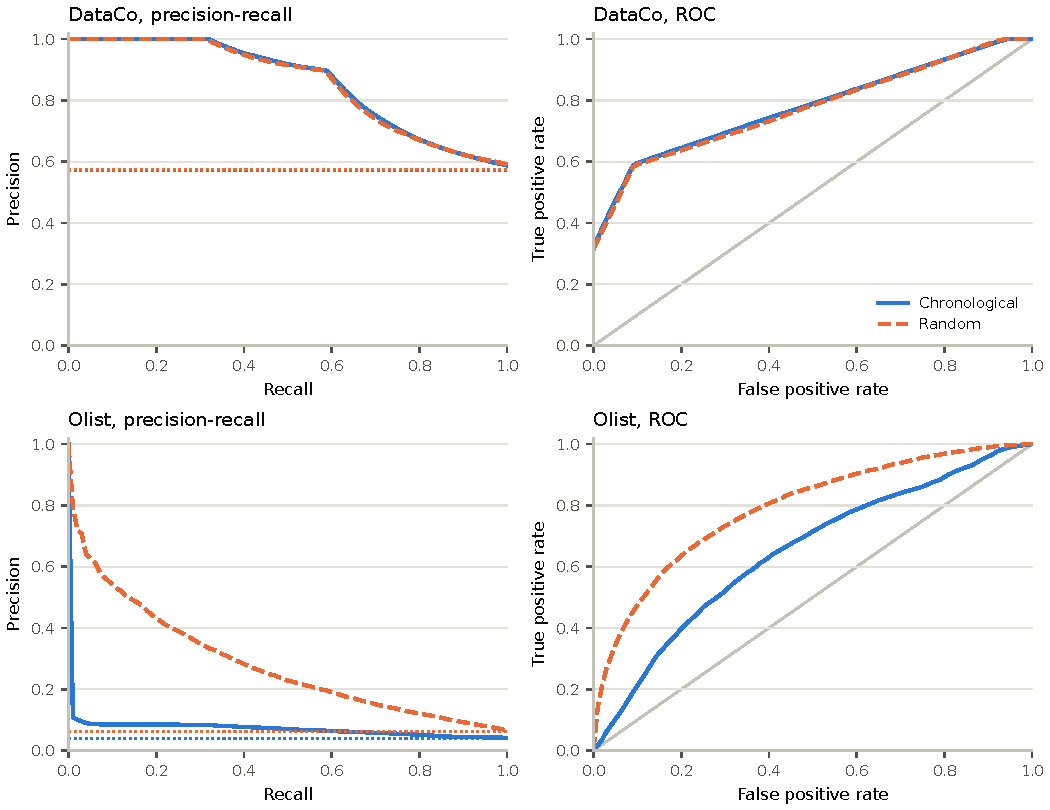
\includegraphics[width=\textwidth]{../figures/courbes_pr_roc_en.pdf}
\caption{Precision-recall (left) and ROC (right) curves of XGBoost on the test set, under the two protocols, averaged over the five seeds. Precision is interpolated: at each recall, the best precision reached at a recall at least as high. The horizontal dotted lines give the prevalence of each test set, that is, the precision of a classifier without discriminating power; the diagonal is the ROC curve of such a classifier.}
\label{fig:courbes}
\end{figure}

\subsection{Monthly performance follows prevalence}
\label{sec:res-derive}

Figure~\ref{fig:derive} breaks the chronological performance down by month. On Olist, the PR-AUC of XGBoost varies from 0.049 in July 2018 to 0.127 in May 2018, and closely follows the monthly prevalence, which ranges from 1.2\% in June to 9.7\% in August. August contains only orders placed up to the 4th, because of the end-of-period truncation (Section~\ref{sec:data-understanding}). This parallel illustrates Equation~\eqref{eq:prec-bayes}: for comparable discriminating power, precision, and with it the PR-AUC, rises and falls with prevalence. On DataCo, the profile is flat: the PR-AUC of XGBoost stays between 0.834 and 0.871 over the nine months of the test period, for a prevalence between 55.8 and 58.7\%. It does not dip after October 2017, despite the change in order structure described in Section~\ref{sec:data-understanding}: this covariate shift has no visible effect on performance.

\begin{figure}[!htbp]
\centering
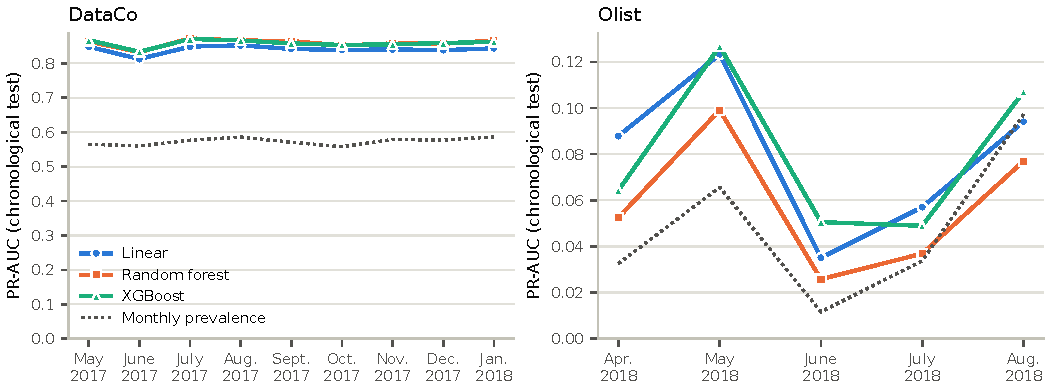
\includegraphics[width=\textwidth]{../figures/profil_derive_en.pdf}
\caption{Drift profile: monthly PR-AUC on the chronological test set, averaged over the five seeds, and monthly prevalence, which is the PR-AUC of a classifier without discriminating power. The vertical scales differ between the two datasets.}
\label{fig:derive}
\end{figure}

\subsection{The protocol reverses the deployment decision}
\label{sec:res-decision}

Table~\ref{tab:decision} and Figure~\ref{fig:economie} answer RQ2. On Olist, in the main scenario $r = 5$, the random protocol credits XGBoost with a saving of 19.6\% over the best policy without a model; the chronological protocol shows that in deployment the same model costs 22.3\% more than that policy. The saving gap is 0.419, with an interval from 0.283 to 0.554. The precision of alerts falls from 0.278 to 0.080: in deployment, more than nine alerts out of ten would be false. The three models lead to the same conclusion, and it becomes sharper as $r$ increases: at $r = 10$, the chronological saving of XGBoost falls to $-$61.4\%, while the random protocol announces $+$34.2\%. For $r = 1$, chronological validation advises never alerting in 93\% of the studies, against 27\% under the random protocol. The evaluation protocol therefore does not merely change a score: it turns the recommendation to deploy the model into a recommendation not to deploy it.

On DataCo, the two protocols agree. For $r = 1$, the models reduce the cost by 32 to 36\% under either protocol. From $r = 2$ onwards, with a majority of late orders, alerting everyone becomes almost optimal: at $r = 5$, the models alert 96 to 100\% of orders and save no more than 6.5\%. The decision value of the models is then limited to the case where both errors cost the same.

\begin{table}[!htbp]
\centering
\footnotesize
\caption{Decision in the main scenario $r = 5$: $F_1$ and saving $S$ (Equation~\eqref{eq:economie}) on the test set, at the threshold chosen on validation, and saving gap $\Delta_S$ with its 95\% interval. \textsuperscript{ns}: the interval contains zero.}
\label{tab:decision}
\begin{tabular}{@{}lccccc@{}}
\toprule
 & \multicolumn{2}{c}{$F_1$} & \multicolumn{2}{c}{Saving $S$} & \\
\cmidrule(lr){2-3}\cmidrule(lr){4-5}
Model & chrono & random & chrono & random & $\Delta_S$ \\
\midrule
\tablerows{tables_en/decision.tex}
\bottomrule
\end{tabular}
\end{table}

\begin{figure}[!htbp]
\centering
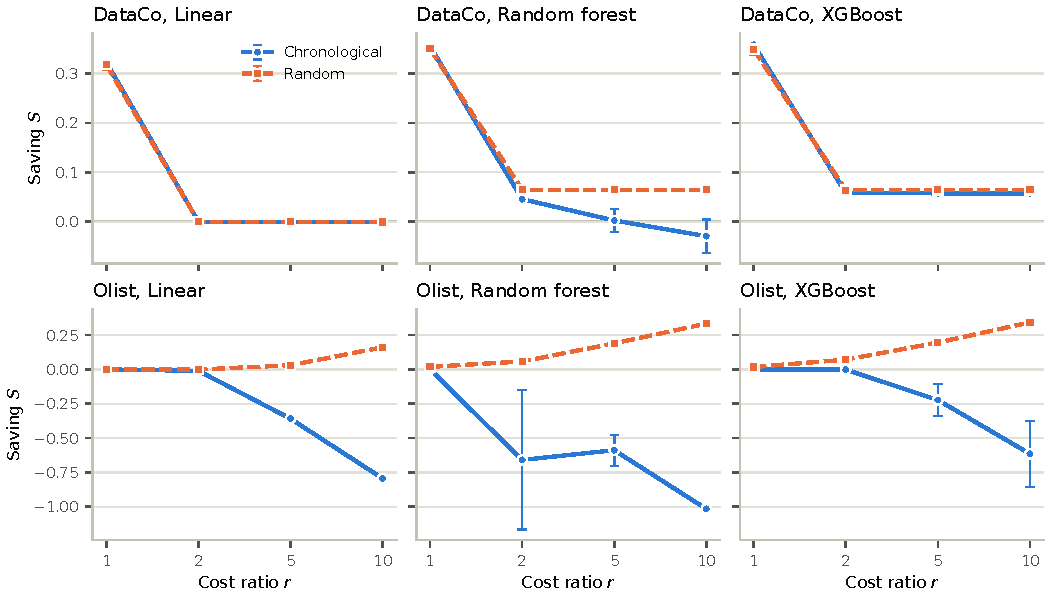
\includegraphics[width=\textwidth]{../figures/economie_cout_en.pdf}
\caption{Saving $S$ relative to the best policy without a model, as a function of the cost ratio $r$, under the two protocols. Mean over the five seeds; the bars give the standard deviation. A negative saving means that the model does worse than the best decision taken without it.}
\label{fig:economie}
\end{figure}

\subsection{The gap depends on the stationarity of the data}
\label{sec:discussion}

\paragraph{Why the two datasets diverge.} The two datasets differ precisely in their stationarity. The prevalence of DataCo varies little from one quarter to the next, and its scheduled lead time is entirely set by the shipping mode (Section~\ref{sec:data-understanding}): the relation between features and delay does not change, and interleaving training and test gives the model no information it does not already have. These regularities also suggest that DataCo is partly generated, which limits its value as a reference dataset. Olist, conversely, shows variations in prevalence from one quarter to the next; the drop in ROC-AUC under the chronological protocol further indicates that the drift is not limited to a prior probability shift (Section~\ref{sec:metriques}). We do not seek to identify the type of drift; the finding is that the optimism gap is not a fixed property of the problem, but depends on the stationarity of the data. A zero gap on one dataset therefore guarantees nothing about another.

\paragraph{Practical relevance.} On Olist, random evaluation would lead to deploying an alert system that costs more than it brings. The chronological protocol, which reproduces deployment conditions, also reveals that the linear baseline is at least as good as the tree ensembles there, which the random protocol hides. The choice of protocol therefore conditions both the decision to deploy and the choice of model.

\paragraph{Threats to validity.} Several limitations frame these results. Each dataset has a single test period: the confidence interval reflects only the variability due to the seeds, not that of the test sample (Section~\ref{sec:partitions}). The costs are illustrative assumptions; the conclusion on Olist nevertheless holds for $r \ge 5$, and, for both tree ensembles, the saving gap is positive for all values of $r$ studied. The policy without a model used as the reference knows the test prevalence, which slightly favours it. On DataCo, the metrics are computed per row and not per order; as an order has a single row from October 2017, the chronological test set weighs more heavily on that period. On Olist, the end-of-period truncation removes the last weeks of purchases. Finally, the gap on the MAE is confounded with the difference in delay distribution between the two test sets, and we do not interpret it.

% ============================================================================
% Section 7: Conclusion
% ============================================================================
\section{Conclusion}
\label{sec:conclusion}

This article examined to what extent the evaluation protocol affects the estimated reliability of delivery delay prediction models when the data distribution changes over time. We compared random and chronological splitting on two public datasets, DataCo and Olist, for the classification of the occurrence of delays and the regression of their magnitude, with a linear baseline, a random forest and XGBoost tuned with an equal budget, under a temporal causality constraint that rules out any information leakage.

\paragraph{Answers to the research questions.} The answer to RQ1 is nuanced: the degradation under temporal evaluation is found on Olist, but not on DataCo. On Olist, whose prevalence of delays varies from one quarter to the next, random splitting strongly overestimates performance: the PR-AUC of XGBoost rises from 0.067 under deployment conditions to 0.279 under random evaluation, and the ROC-AUC, which does not depend on prevalence, falls as well. On DataCo, whose prevalence stays stable, the two protocols give equivalent estimates. The optimism gap is therefore not a fixed property of the problem: it depends on the stationarity of the data, and a zero gap on one dataset guarantees nothing about another. The answer to RQ2 is clear for Olist: in the main cost scenario, the random protocol credits the model with a saving of 19.6\% over the best policy without a model, whereas the chronological protocol shows that it would cost 22.3\% more. The evaluation protocol thus turns the recommendation to deploy the alert system into a recommendation not to deploy it.

\paragraph{Contributions.} We proposed a model comparison based on a protocol that rules out any temporal leakage, including in the history features and in the tuning folds; a measure of the optimism gap between protocols, together with a confidence interval, a monthly drift profile and its translation into decision cost; and a check of these results on two independent datasets, which shows that the gap depends on the data. The whole pipeline, from raw data to result tables, is reproducible through a sequence of \texttt{make} commands; the code and results are available at \url{https://github.com/Juan-Lucas/supply_chain_resilience}.

\paragraph{Recommendations.} For delay prediction, and more broadly for any operational prediction whose data are ordered in time, we recommend evaluating models with a chronological split, tuning their hyperparameters on folds that respect the same order, reporting the prevalence of each evaluated period, and translating performance into decision cost rather than relying on a ranking metric alone. A random evaluation is defensible only after checking that the data are stationary.

\paragraph{Limitations and future work.} Our conclusions rest on a single test period per dataset, on illustrative costs and on two datasets, one of which is probably partly generated (Section~\ref{sec:discussion}). Several extensions follow. Repeating the evaluation over several successive test periods would measure the variability due to the test sample, which our intervals do not include. Company data recording the actual costs of delays and alerts would make the decision analysis less dependent on assumptions. Finally, the weakness of the models on Olist under deployment conditions calls for studying periodic retraining and drift detection, as well as features able to capture changes in logistics load.

% ============================================================================
% Bibliography
% ============================================================================
\bibliographystyle{plain}
\bibliography{related_work}

\end{document}
